\documentclass{article}

\title{Zarządzanie i harmonogramowanie procesów - zadanie 2}
\author{Artur Dziedziczak 315900}
\date{\today}

\usepackage{subcaption}
\usepackage{microtype}
\usepackage[
    backend=biber,
    natbib=true,
    url=true,
    doi=true,
    eprint=false
]{biblatex}
\usepackage[a4paper, total={6in, 8in}]{geometry}

\addbibresource{sample.bib}
\usepackage{gensymb}
\usepackage{graphicx}

\usepackage{hyperref}
\hypersetup{
    colorlinks=true,
    linkcolor=blue,
    filecolor=magenta,
    urlcolor=cyan,
    pdftitle={Zarządzanie i harmonogramowanie procesów - Zad. 1 Artur Dziedziczak 315900},
    pdfpagemode=FullScreen,
    }

\usepackage{float}

\usepackage[utf8]{inputenc}
\usepackage{amsthm}
\usepackage{enumitem}
\usepackage[english, polish]{babel}
\usepackage[T1]{fontenc}
\usepackage{theorem}
\usepackage{listings}

\lstset{frame=tb,
  language=Bash,
  aboveskip=3mm,
  belowskip=3mm,
  showstringspaces=false,
  columns=flexible,
  basicstyle={\small\ttfamily},
  numbers=none,
  numberstyle=\tiny\color{gray},
  keywordstyle=\color{blue},
  commentstyle=\color{dkgreen},
  stringstyle=\color{mauve},
  breaklines=true,
  breakatwhitespace=true,
  tabsize=3
}

\usepackage[justification=centering]{caption}
\begin{document}

\maketitle

\section {Szeregowanie zadań na jednakowych procesorach równoległych}
\subsection{Zadania podzielne}

Na podstawie podanych danych \(n\) - liczba procesów,
\(p_j\) - czas wykonania \(j\)-tego zadania, określić minimalny czas,

w jakim można zakończyć wszystkie zadania (\(C_{max}\)).
Stworzyć harmonogram realizujący wyznaczony czas.

Przedstawiony problem jest to problem P2|pmtn|Cmax to znaczy problem szeregowania podzielnych i niezależnych zadań na dwóch procesorach z kryterium $C_{max}$.

Można je zamodelować w GLPK w następujący sposób.

\noindent Model matematyczny: \\\\

\noindent Identyfikacja zbiorów:

$T_j$ - zadania do wykonania $j = {A,B,C,D,E,F,G,H}$

$L_{l}$ - procesor na którym wykonywane są zadania $l = {1,2}$

\noindent Parametry modelu:

$p_{jl}$ - czas wymagany do wykonania zadania $p_j$ na procesorze $l$ gdzie $j = {A,B,C,D,E,F,G,H}$, $l = {1,2}$

\noindent Zmienne decyzyjne:

$C_{max}$ - zmienna określająca maksymalny czas pracy maszyny
$x_{jl}$ - czas wykonywania zadania $x_j$ na procesorze $l$ gdzie $j = {A,B,C,D,E,F,G,H}$, $l = {1,2}$

\noindent Funkcja celu:

$min C_{max}$ - maksymalny czas zakończenia

\noindent Ograniczenia:

$\sum^{j}_{l = 1} x_{jl} = p_j$ - każde zadania jest musi trwać przez podany czas 

$\sum^{l}_{j = 1} x_{jl} <= C_{max}$ - każda maszyna może pracować przez najwyżej $C_{max}$

$\sum^{j}_{l = 1} x_{jl} <= C_{max}$ - wartość $C_{max}$ jest najwyższa ze wszystkich czasów przetwarzania $p_j$

\lstinputlisting[
language=AMPL,
numbers=left,
firstnumber=1,
caption={Kod solvera zad1a.mod},
aboveskip=10pt,
]
{glpsol/zad1a.mod}

\lstinputlisting[
language=AMPL,
numbers=left,
firstnumber=1,
caption={Kod wynikowy solvera zad1a.mod},
aboveskip=10pt,
]
{glpsol/zad1a.output}

Jak widać solver znalazł minimalny czas w jaki można zakończyć wszystkie zadania $41$ jednostek czasu.

Dla tego rozwiązania wytworzyłem również harmonogram.

\begin{figure}[h]    
  \centering    
  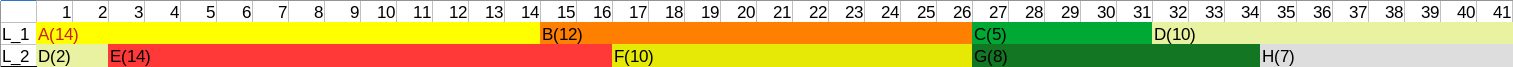
\includegraphics[width=\linewidth]{others/zad1a_harmonogram.png}
  \caption{Harmonogram dla zad1a}
\end{figure}

Jak widać zadanie $D$ zostało podzielone na 2 procesory.

\subsection{Zadania niepodzielne}

\begin{enumerate}[label=(\alph*)]
    \item \label{12a} Mając dane: (n) - liczba procesów, $(p_j)$ - czas wykonania
          $(j)$-tego zadania, stworzyć model minimalizujący czas wykonania
          wszystkich zadań ($(C_{max}$)). Porównać wynik z rozwiązaniem,
          gdy zadania były podzielne.
          Jaka zależność zachodzi w ogólnym przypadku między rozwiązaniami tych zadań?
  \item \label{12b} Zaproponować regułę przydziału zadań minimalizującą czas
          wykonania wszystkich zadań ($(C_{max}$)).
          Porównać wynik z rozwiązaniem optymalnym - jaka zależność zachodzi w ogólnym przypadku?
  \item \label{12c} Mamy Rozwiązanie - niekoniecznie optymalne. Zaproponuj algorytm lokalnej poprawy rozwiązania.
\end{enumerate}

\par\noindent\rule{\textwidth}{0.4pt}
Odpowiedź \ref{12a}
\par\noindent\rule{\textwidth}{0.4pt}

Zadanie \ref{12a} jest to problem $P2||C_{max}$ czyli dotyczy zadań niepodzielnych na dwóch procesorach z kryterium $C_{max}$. W jego rozwiązaniu wykorzystuje się szeregowanie listowe.

\noindent Model matematyczny: \\\\

\noindent Identyfikacja zbiorów:

$T_j$ - zadania do wykonania $j = {A,B,C,D,E,F,G,H}$

$L_{l}$ - procesor na którym wykonywane są zadania $l = {1,2}$

\noindent Parametry modelu:

$p_{j}$ - czas wymagany do wykonania zadania $j = {A,B,C,D,E,F,G,H}$

\noindent Zmienne decyzyjne:

$C_{max}$ - zmienna określająca maksymalny czas pracy maszyny
$x_{lj}$ - macierz przydziału procesora. Zawiera wartości binarne $j = {A,B,C,D,E,F,G,H}$, $l = {1,2}$ 

\noindent Funkcja celu:

$min C_{max}$ - maksymalny czas zakończenia

\noindent Ograniczenia:

$\sum^{l}_{j = 1} x_{jl} * p_j <= C_{max}$ - każda maszyna może pracować przez najwyżej $C_{max}$

$\sum^{j}_{l = 1} x_{jl} = 1$

$x_{jl} \in {0,1}$

\lstinputlisting[
language=AMPL,
numbers=left,
firstnumber=1,
caption={Kod solvera zad12a.mod},
aboveskip=10pt,
]
{glpsol/zad12a.mod}

\lstinputlisting[
language=AMPL,
numbers=left,
firstnumber=1,
caption={Kod wynikowy solvera zad12a.mod},
aboveskip=10pt,
]
{glpsol/zad12a.output}

Jak widać solver znalazł rozwiazązanie $41$ jednostek czasu oraz macierz przydziału procesora. Macierz tę prezentuje na poniższym harmonogramie.

\begin{figure}[h]    
  \centering    
  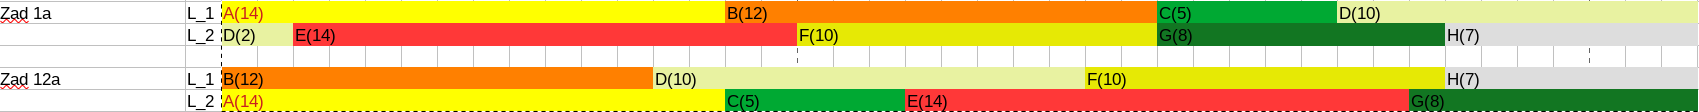
\includegraphics[width=\linewidth]{others/zad12a_harmonogram.png}
  \caption{Harmonogram dla zad12a}
\end{figure}

Widać na nim, że zadanie $D$ nie zostało podzielone a zmiana zadań $A, C, D$ na drugi procesor spowodowała, że czas
wykonania wszystkich zadań nie zmienił się.

\par\noindent\rule{\textwidth}{0.4pt}
Odpowiedź \ref{12b}
\par\noindent\rule{\textwidth}{0.4pt}

Odpowiedzią na \ref{12b} jest użycie szeregowania listowego z zasadą LPT. Metoda ta pozwala na wybieranie zadań w kolejności zgodnej z wyznaczona listą priorytetów zadań. W kolejnych krokach metody, jeśli w danej chwili jakieś procesory są wolne, to wybierane jest pierwsze zadanie oczekujace na liście i jest przydzielane do procesora gwarantującego najwcześniejszy termin ukończenia tego zadania. Jako, że w podanym zadaniu nie ma uwzględnionych priorytetów to wykorzystywana jest reguła LPT (ang. Longest Processsing Time).

\par\noindent\rule{\textwidth}{0.4pt}
Odpowiedź \ref{12c}
\par\noindent\rule{\textwidth}{0.4pt}

Jeżeli mamy rozwiązanie nikoniecznie optymalne \ref{12c} należy wykorzystać metodę LPT, która z definicji podanej w wykładzie \textbf{W przypadku Problemu $P||C_{max}$ najlepszy wartiant algorytmu szeregowania listowego LS wykorzystuje regułę priorytetową LPT. Wtedy długość uszeregowania $C_{max}$ jest w najgorszym przypadku nie gorsza od optymalnej wartości $C_{max}$ co najwyżej ($\frac{4}{3} - \frac{1}{3m}$) razy.}

\section{Szeregowanie zadań na niejednorodowych procesorach równoległych}

\begin{table}[H]
	\centering
	\begin{tabular}{| c | c | c |}
		\hline
		Zadanie & Czas obsługi na 1. procesorze - $(p_{1j}$) & Czas obsługi na 2. procesorze - $(p_{2j}$) \\
		\hline
		A       & 14                                         & 9                                          \\
		B       & 14                                         & 16                                         \\
		C       & 5                                          & 8                                          \\
		D       & 11                                         & 9                                          \\
		E       & 14                                         & 12                                         \\
		F       & 12                                         & 16                                         \\
		G       & 8                                          & 5                                          \\
		H       & 9                                          & 17                                         \\
		\hline
	\end{tabular}
	\caption{Czas obsługi na poszczególnych procesorach}
	\
\end{table}

\subsection{Zadania podzielne \label{21}}
Mając dane \(p_{ij}\) — czas wykonania \(j\)-tego zadania na \(i\)-tym procesorze,
zaproponuj model minimalizujący czas wykonania wszystkich zadań (\(C_{max}\)).

\par\noindent\rule{\textwidth}{0.4pt}
Odpowiedź \ref{21}
\par\noindent\rule{\textwidth}{0.4pt}

\ref{21} Jest to problem $R|pmtn|C_{max}$ czyli rozważany jest problem szeregowania $n$ zadań niezależnych i podzielnych na $m$ procesorach równoległych. $n = 8$, $m = 2$.

Można go zamodelować w następujący sposób.

\noindent Model matematyczny: \\\\

\noindent Identyfikacja zbiorów:

$T_j$ - zadania do wykonania $j = {A,B,C,D,E,F,G,H}$

$L_{l}$ - procesor na którym wykonywane są zadania $l = {1,2}$

\noindent Parametry modelu:

$p_{lj}$ - czas przetwarzania zadania $j$ na maszynie $l$ gdzie $j = {A,B,C,D,E,F,G,H}$, $l = {1,2}$

\noindent Zmienne decyzyjne:

$x_{jl}$ - czas w jakim zadanie $j$ jest przetwarzane na mszynie $l$ gdzie $j = {A,B,C,D,E,F,G,H}$, $l = {1,2}$ 
$C_{max}$ - zmienna określająca czas zakończenia wszystkich zadań

\noindent Funkcja celu:

$min C_{max}$ - minimalny czas zakończenia

\noindent Ograniczenia:

Ograniczenia przpisane z ksiązki \cite{scheduling}.

$\sum^{l}_{j = 1} \frac{x_{lj}}{p_{lj}} = 1$ - każda operacja musi być w pełni wykonana

$\sum^{j}_{l = 1} x_{lj} <= C_{max}$  - czas pracy zadania na wszystkich maszynach

$\sum^{l}_{j = 1} x_{lj} <= C_{max}$  - maksymalny czas pracy mszyny dla wszystkich zadań

\lstinputlisting[
language=AMPL,
numbers=left,
firstnumber=1,
caption={Kod solvera zad21.mod},
aboveskip=10pt,
]
{glpsol/zad21.mod}

\lstinputlisting[
language=AMPL,
numbers=left,
firstnumber=1,
caption={Kod wynikowy solvera zad21.mod},
aboveskip=10pt,
]
{glpsol/zad21.output}

Solver rozwiązał problem i określił, że wykonanie zadań zajmie w przybliżeniu $37.7$ jednostek czasu.

\subsection{Zadania niepodzielne}
\begin{enumerate}[label=(\alph*)]
    \item \label{22a} Mając dane $(p_{ij})$ — czas wykonania j-tego zadania na i-tym procesorze,
          zaproponuj model minimalizujący czas wykonania wszystkich
          zadań ($(C_{max})$).
    \item \label{22b} Mając dane $(p_{ij})$ — czas wykonania j-tego zadania na i-tym procesorze,
          zaproponuj model minimalizujący sumę czasów przebywania w
          systemie ($(\sum F_j$))
    \item \label{22c} czas wykonania j-tego zadania na i-tym procesorze,
          zaproponuj model minimalizujący sumę czasów oczekiwania na obsługę.
          (Wskazówka - czym różni ten punkt od poprzedniego)
\end{enumerate}

\par\noindent\rule{\textwidth}{0.4pt}
Odpowiedź \ref{22a}
\par\noindent\rule{\textwidth}{0.4pt}

Przedstawiony w zadaniu \ref{22a} problem sprowadza się do znalezienia optymalnej alokacji zadań procesorów dla zadań niepodzielnych.

Można go przedstawić za pomocą programowania liniowego.

\noindent Model matematyczny: \\\\

\noindent Identyfikacja zbiorów:

$T_j$ - zadania do wykonania $j = {A,B,C,D,E,F,G,H}$

$L_{l}$ - procesor na którym wykonywane są zadania $l = {1,2}$

\noindent Parametry modelu:

$p_{lj}$ - czas przetwarzania zadania $j$ na maszynie $l$ gdzie $j = {A,B,C,D,E,F,G,H}$, $l = {1,2}$

\noindent Zmienne decyzyjne:

$x_{jl}$ - czas w jakim zadanie $j$ jest przetwarzane na mszynie $l$ gdzie $j = {A,B,C,D,E,F,G,H}$, $l = {1,2}$ 
$C_{max}$ - zmienna określająca czas zakończenia wszystkich zadań

\noindent Funkcja celu:

$min C_{max}$ - minimalny czas zakończenia

\noindent Ograniczenia:

Ograniczenia przpisane z podręcznika.

$\sum^{l}_{j = 1} p_{lj}*x{lj} <= C_{max}$

$\sum^{j}_{l = 1} x_{lj} = 1$

$x_{lj} \in {0,1}$

\lstinputlisting[
language=AMPL,
numbers=left,
firstnumber=1,
caption={Kod solvera zad22a.mod},
aboveskip=10pt,
]
{glpsol/zad22a.mod}

\lstinputlisting[
language=AMPL,
numbers=left,
firstnumber=1,
caption={Kod wynikowy solvera zad22a.mod},
aboveskip=10pt,
]
{glpsol/zad22a.output}

Znaleziony przez solver czas to $40$ jednostek. Poniżej przedstawiam znaleziony harmonogram.

\begin{figure}[h]    
  \centering    
  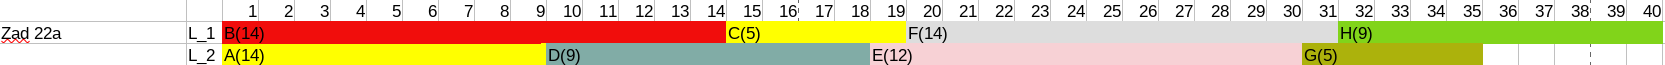
\includegraphics[width=\linewidth]{others/zad22a_harmonogram.png}
  \caption{Harmonogram dla zad22a}
\end{figure}

\par\noindent\rule{\textwidth}{0.4pt}
Odpowiedź \ref{22b}
\par\noindent\rule{\textwidth}{0.4pt}



\printbibliography
\end{document}
